\section{Results}
\subsection{Initial Analysis}
We discovered that the front-end languages react and angular received a disproportionate number of commits during the initial analysis. These data show a distinct trend in language usage over time, with the number of commits for react decreasing from the year 2015, which was 2656, to the year 2021, which was 778, and the same is valid for angular.
In 2015, there were 3364 commits, and by 2021, that number will have dropped to 2278.

Compared to other front end languages, these two languages received the most significant number of commits because they were both the most ancient languages. During those years, most front-end applications relied solely on these programming languages to achieve their functionality.

The vue language had the lowest number of commits compared to all other languages. This is because it is a new developing language and people are more familiar with the front end languages they use from the beginning.

According to the data in all of the graphs, the number of open issues for Angular was the highest compared to all other languages, and the same was true for the number of closed issues. When it comes to frontend languages, Angular is most commonly used, and a wide range of applications supports it. Despite this, the number of open issues for new languages has increased in the years following 2019. We can assume that people started working on these languages because they offer better scalability, performance, security, and other advantages over react and angular.

\subsection{Answers}
\subsubsection{Is the project alive?}
We are going to use \textbf{time} as the basis to which we are going to attach the metrics, if we see an increase overtime around a project we could say that a project has an active community and the contributions, which could be issues or commits, are increasing over time, otherwise if we see a decline we can see how steep this decline is, and raise that so the contributor take that into consideration.

\paragraph{Trend of commits over the years}
\begin{center}
    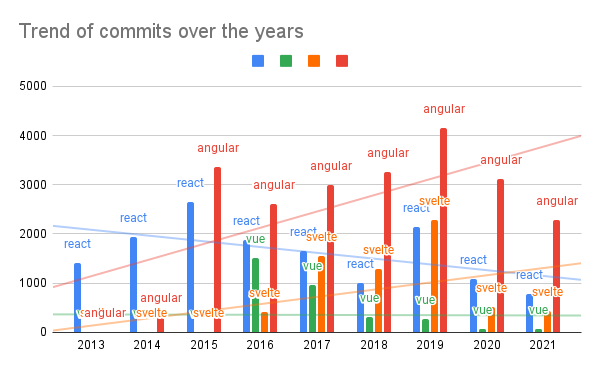
\includegraphics[scale=0.38]{trend-of-commits-over-the-years}    
\end{center}
We use the following data set 
\paragraph{Trend of opened issues over the years}
\paragraph{Trend of issues by state}
\paragraph{Trend of unique contributors per year}
\paragraph{Trend of comments by year}


\subsubsection{What is the overall sentiment of the project?}
